\documentclass[a4paper]{article}

\usepackage[margin=1in]{geometry} 
\usepackage{amsmath,amsthm,amssymb}
\usepackage{amssymb}
\usepackage{float}
\usepackage{graphicx}
\usepackage{xcolor}
\usepackage[UKenglish]{isodate}
\origdate
\cleanlookdateon
\usepackage[utf8]{inputenc}
\usepackage[hidelinks]{hyperref}
\usepackage{tikz-cd}
\usepackage{enumitem}
\usepackage{mathtools}
\usepackage{pgfplots}
\usepackage{float}
\usepackage{tikz, venndiagram}
\usepackage{tkz-euclide}
\usepackage{tabu}
\usepackage{framed}
\usepackage{steinmetz}
\usepackage{wasysym}
\usepackage{forest}
\usepackage{mathrsfs}
\renewcommand{\baselinestretch}{1.5} 
\newcommand*\mycirc[1]{%
  \begin{tikzpicture}
      \node[draw,circle,inner sep=1pt] {#1};
   \end{tikzpicture}}
%%% Better lambda 
\usepackage{pifont}
\usepackage{kpfonts}
\makeatletter
\newcommand\Pimathsymbol[3][\mathord]{%
  #1{\@Pimathsymbol{#2}{#3}}}
\def\@Pimathsymbol#1#2{\mathchoice
  {\@Pim@thsymbol{#1}{#2}\tf@size}
  {\@Pim@thsymbol{#1}{#2}\tf@size}
  {\@Pim@thsymbol{#1}{#2}\sf@size}
  {\@Pim@thsymbol{#1}{#2}\ssf@size}}
\def\@Pim@thsymbol#1#2#3{%
  \mbox{\fontsize{#3}{#3}\Pisymbol{#1}{#2}}}
\makeatother
% the next two lines are needed to avoid LaTeX substituting upright from another font
\input{utxmia.fd}
\DeclareFontShape{U}{txmia}{m}{n}{<->ssub * txmia/m/it}{}
% you may also want
\DeclareFontShape{U}{txmia}{bx}{n}{<->ssub * txmia/bx/it}{}
% just in case
%\DeclareFontShape{U}{txmia}{l}{n}{<->ssub * txmia/l/it}{}
%\DeclareFontShape{U}{txmia}{b}{n}{<->ssub * txmia/b/it}{}
% plus info from Alan Munn at https://tex.stackexchange.com/questions/290165/how-do-i-get-a-nicer-lambda?noredirect=1#comment702120_290165
\newcommand{\pilambdaup}{\Pimathsymbol[\mathord]{txmia}{21}}
\pgfplotsset{compat=1.16}
\begin{document}
\title{Midterms Revision Guide\\[0.1cm]
    \large 30.101 Systems \& Control, Term 5 2020}
\author{Wei Min Cher}
\date{06 Mar 2020}

\maketitle

\tableofcontents

\newpage
\section{W1: Linear Time-Invariant Systems}
\subsection{Signals}
\begin{itemize}
    \item Signal: function changing in time and space
\end{itemize}
Continuous signal e.g. $x(t), \ -\infty<t<\infty$\\
Discrete signal e.g. $x[k], \ k = 1, 2,\ldots$\\
Determinstic signal e.g. $x(t) = \cos\omega t$ \quad exact value of x(t) at any t is known\\
Random/stochastic signal e.g $x(t) = \cos(\omega t+ \phi), \ \phi=\{0, \frac{\pi}{2}, \pi\}$ \quad esact value of x(t) at any t is unknown\\
Periodic signal e.g. $x(t) = \sin t$, where $x(t) = x(t+T)$\\
Non-periodic signal e.g. $x(t) = \begin{cases}
\quad\cos t, & t < 0\\
\quad\sin t, & t \geq 0\\
\end{cases}$\quad , where $x(t) \neq x(t+T)$\\
Bounded signal: $x(t)\text{ does not}\rightarrow \infty$ as $t\rightarrow\infty$\\
Unbounded signal: $x(t)\rightarrow\infty\text{ as }t\rightarrow\infty$
\subsubsection{Basic signals}
\begin{enumerate}[label=\alph*.]
    \item Unit impulse function $\delta(t)$
        \begin{align*}
            \delta(t) &= \begin{cases}
            \quad \infty, & t = 0\\
            \quad 0, & t \neq 0
            \end{cases}
            \hspace{2cm} \int_{0^-}^{0^+}\delta(t) \ dt = 1
        \end{align*}
    \item Unit step function $u(t)$
        \begin{align*}
            u(t) = \begin{cases}
            \quad 1, & t \geq 0\\
            \quad 0, & t < 0
            \end{cases}
        \end{align*}
    \item Rectangular function $\text{rect}\left(\frac{t}{T}\right)$
    \begin{align*}
        \text{rect}\left(\frac{t}{T}\right) &= \begin{cases}
        \quad 1, & -\frac{T}{2} < t < \frac{T}{2}\\
        \quad 0, & \text{elsewhere}
        \end{cases}\\
        &= u\left(t+\frac{T}{2}\right) - u\left(t-\frac{T}{2}\right)
    \end{align*}
    \item Exponential growth/decay function
    $$x(t) = Ce^{at}$$
    \begin{itemize}
        \item Exponential growth: $C>0$
        \item Exponential decay: $C<0$
    \end{itemize}
\end{enumerate}
\subsection{System Properties}
\begin{enumerate}
    \item Causal: output depends on input at present, past
    \item Linearity: has property of superposition
    \item Time Invariance: time shift in output = time shift in inuput
\end{enumerate}
\subsection{Complex exponential sinusoidal signals}
\begin{itemize}
    \item $\sin(\omega t) = \displaystyle\frac{1}{2j}\left(e^{j\omega t}-e^{-j\omega t}\right)$
    \item $\cos(\omega t) = \displaystyle\frac{1}{2}\left(e^{j\omega t}+e^{-j\omega t}\right)$
    \item $e^{\pm j\theta} = \cos\theta \pm j \sin\theta$
\end{itemize}
\subsection{Zeros and Poles}
\begin{itemize}
    \item General form of G(s): $$G(s) = \frac{K(s+z+1)(s+z_2)\cdots(s+z_m)}{(s+p_1)(s+p_2)\cdots(s+p_n)}=\frac{\text{N(s)}}{\text{D(s)}},$$
    \begin{center}
       where N(s) is a polynomial of degree m and D(s) is a polynomial of degree n, and m $<$ n.
    \end{center}
    \begin{itemize}[label=$\circ$]
        \item Zeros ($\ocircle$): points where N(s) = 0
        \quad e.g. $s=-z_1, -z_2,\cdots,-z_m$
        \item Poles/roots ($\times$): points where D(s) = 0 \quad e.g. $s=-p_1, -p_2, \cdots, -p_n$
    \end{itemize}
\end{itemize}
\subsection{Differential equations}
\begin{center}
\boxed{
\begin{forest}
 [Differential Equations
 [Ordinary
 [Linear
 [Time Invariant]
 [Time Varying]
 ]
 [Non-linear]
 ]
 [Partial]
 ]
\end{forest}
}
\end{center}
\subsubsection{Ordinary Differential Equations (ODEs)}
\begin{itemize}
    \item General form:
    $$g\left(\frac{d^n x}{dt^n},\frac{d^{n-1}x}{dt^{n-1}},\cdots, x, t\right) = f(t)$$
    \begin{itemize}[label=$\circ$]
        \item where $x$ is the dependent variable;
        \item $t$ is the independent variable.
    \end{itemize}
    \item Linear ODE: output and its derivatives are pure functions of input, and are to power 1
    \item Non-linear ODE: output and its derivatives are not pure functions of input
    \item Time Invariant ODE: coefficients are independent of $t$
    \item Time Varying ODE: coefficients are functions of $t$
\end{itemize}
\subsection{Laplace Transform (LT)}
If $f(t) = 0$ for $t<0$:
\begin{align*}
    F(s) = \mathscr{L}[f(t)] = \int_{0}^{\infty}f(t)e^{-st}\ dt, \ t\geq 0
\end{align*}
\begin{itemize}
    \item where $s=\sigma +j\omega$
    \item $\displaystyle \int_0^\infty$ is an improper integral, thus Laplace Transform may not exist
    \begin{itemize}[label=$\circ$]
        \item Laplace Transform exists within Region of Convergence (ROC)
    \end{itemize}
\end{itemize}
\subsection{Initial Value Theorem}
If $f(t)$ and $\displaystyle\frac{df(t)}{dt}$ are both Laplace Transformable and $\displaystyle\lim_{s\rightarrow\infty} sF(s)$ exists,
\begin{align*}
    f(0^+) = \lim_{s\rightarrow\infty} sF(s)
\end{align*}
\subsection{Final Value Theorem}
If $f(t)$ and $\frac{df(t)}{dt}$ are Laplace Transformable and $\displaystyle\lim_{t\rightarrow\infty} f(t)$ exists,\\
and $sF(s)$ has all its poles with \textcolor{red}{\textbf{strictly negative real part}},
\begin{align*}
    f(\infty) = \lim_{s\rightarrow0} sF(s)
\end{align*}
\subsection{Inverse Laplace Transform (ILT)}
\begin{enumerate}
    \item Express $F(s)$ as a proper rational fraction: $\displaystyle F(s) = \frac{N(s)}{D(s)}$, where degree of $N(s) < D(s)$
    \item Check roots of D(s):
    \begin{enumerate}[label=\large\protect\textcircled{\small\Alph*}]
        \item Roots are Real and Distinct
        \begin{center}
        $\displaystyle F(s) = \frac{N(s)}{D(s)} = \frac{a}{s+p_1}+\frac{a}{s+p_2}+\cdots+\frac{a}{s+p_n},$
        \vspace{0.25cm}\\ 
        $\text{where } a_i = (s+p_i)F(s)|_{s=-p_i}$
        \end{center}
        \item Roots are Real and Repetitive
        \begin{center}
            $\displaystyle F(s) = \frac{b_1}{s+p}+\frac{b_2}{(s+p)^2}+\cdots+\frac{b_n}{(s+p)^n}$
            \vspace{0.25cm}\\ 
            $\text{where }b_i = \displaystyle\frac{1}{(n-1)!}\left[\left.\frac{d^{n-i}}{ds^{n-i}}(s+p)^n F(s)\right]\right|_{s=-p}$
        \end{center}
        \item Roots are Complex Conjugates
        \begin{center}
            $\displaystyle F(s) = \frac{N(s)}{s^2+cs+d} = C_1\frac{\omega}{(s+a)^2+\omega^2}+C_2\frac{s+a}{(s+a)^2+\omega^2}$
            \vspace{0.25cm}\\
            $\displaystyle\text{where poles, }s = -\frac{c}{2}\pm\frac{\sqrt{c^2-4d}}{2} $
        \end{center}
        \item Combination of Cases \large\protect\textcircled{\small A}, \large\protect\textcircled{\small B}, \large\protect\textcircled{\small C}\normalfont
        \begin{itemize}
            \item \normalsize Rewrite numerator in terms of denominator to simplify
        \end{itemize}
    \end{enumerate}
    \item Use Laplace Transform table pairs to infer $f(t)$ from $F(s)$.
\end{enumerate}
\section{W2: Convolution}
\tikzset{every picture/.style={line width=0.75pt}} %set default line width to 0.75pt        
\begin{center}
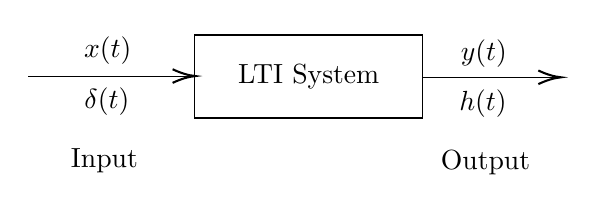
\begin{tikzpicture}[x=0.75pt,y=0.75pt,yscale=-1,xscale=1]
%uncomment if require: \path (0,300); %set diagram left start at 0, and has height of 300

%Shape: Rectangle [id:dp0719812338987873] 
\draw   (140.8,99.8) -- (250.46,99.8) -- (250.46,139.8) -- (140.8,139.8) -- cycle ;
%Straight Lines [id:da4531798525533779] 
\draw    (60.5,119.6) -- (129.02,119.6) -- (139,119.6) ;
\draw [shift={(141,119.6)}, rotate = 180] [color={rgb, 255:red, 0; green, 0; blue, 0 }  ][line width=0.75]    (10.93,-3.29) .. controls (6.95,-1.4) and (3.31,-0.3) .. (0,0) .. controls (3.31,0.3) and (6.95,1.4) .. (10.93,3.29)   ;
%Straight Lines [id:da11632608599684824] 
\draw    (250.46,120.2) -- (315.2,120.2) ;
\draw [shift={(317.2,120.2)}, rotate = 180] [color={rgb, 255:red, 0; green, 0; blue, 0 }  ][line width=0.75]    (10.93,-3.29) .. controls (6.95,-1.4) and (3.31,-0.3) .. (0,0) .. controls (3.31,0.3) and (6.95,1.4) .. (10.93,3.29)   ;

% Text Node
\draw (98.8,107.4) node   [align=left] {$\displaystyle x( t)$};
% Text Node
\draw (98.4,131.8) node   [align=left] {$\displaystyle \delta ( t)$};
% Text Node
\draw (195.63,119.8) node   [align=left] {LTI System};
% Text Node
\draw (280,108.6) node   [align=left] {$\displaystyle y( t)$};
% Text Node
\draw (279.6,133) node   [align=left] {$\displaystyle h( t)$};
% Text Node
\draw (97.2,160.6) node   [align=left] {Input};
% Text Node
\draw (280.8,161.4) node   [align=left] {Output};
\end{tikzpicture}
\end{center}
\subsection{Properties of impulse function}
\begin{enumerate}
    \item $x(t)\delta(t-t_0) = x(t_0)\delta(t-t_0)$
    \item $\displaystyle\int_{-\infty}^{\infty} x(t)\delta(t-t_0)\ dt = x(t_0)$
\end{enumerate}
\subsection{Convolution integral}
$$y(t) = \int_{-\infty}^{\infty}x(\tau)h(t-\tau)\ d\tau\Longleftrightarrow\int_{-\infty}^{\infty}x(t-\tau)h(\tau)\ d\tau$$
\begin{itemize}
    \item It can be written as $y(t) = x(t)*h(t)$
\end{itemize}
\subsection{Graphical Method}
\begin{enumerate}
    \item Flip: $h(\tau)\rightarrow h(-\tau)$
    \item Shift by $t$: $h(-\tau)\rightarrow h(t-\tau)$
    \item Multiply by $x$: $x(\tau)h(t-\tau)$
    \item Integrate over $\tau$: $\displaystyle y(t) = \int_{-\infty}^{\infty}x(\tau)h(t-\tau)\ d\tau$
\end{enumerate}
\subsection{Properties of Convolution}
\begin{itemize}
    \item Commutative: $x(t)*h(t) = h(t)*x(t)$
    \item Associative: $[x(t)*h_1(t)]*h_2(t) = x(t)*[h_1(t)*h_2(t)]$
    \item Distributive: $x(t)*h_1(t)+x(t)*h_2(t) = x(t)*[h_1(t)+h_2(t)]$
\end{itemize}
\newpage
\section{W3: Fourier Analysis}
\subsection{Fourier Series}
$$x(t) = \sum_{k=-\infty}^{\infty}a_k e^{jk\omega_0 t},\ \omega_0 = \frac{2\pi}{T_0}$$
Synthesis: \boxed{x(t) =\sum_{k=-\infty}^{\infty}a_k e^{jk\omega_0 t}}\\
Analysis: \boxed{a_k = \frac{1}{T_0}\int_{T_0}x(t)e^{-jk\omega_0 t}\ dt}
\subsection{Convergence Conditions (Dirichlet Conditions)}
\begin{enumerate}
    \item Signal is integral over any period. \quad $\displaystyle \int_{T_0}|x(t)|<\infty$
    \item Signal must be bounded. \quad $x(t) \text{ cannot be }\pm\infty.$
    \item Finite number of discontinuities in interval $T$.
\end{enumerate}
\subsection{Forms of Fourier Series}
\begin{enumerate}
    \item $\displaystyle x(t) =\sum_{k=-\infty}^{\infty}a_k e^{jk\omega_0 t}$
    \item $\displaystyle x(t) = a_0 + 2\sum_{k=1}^{\infty}A_k\cos(k\omega_0 t+\theta_k)$
    \item $\displaystyle x(t) = a_0 + 2\sum_{k=1}^{\infty}[B_k\cos k\omega_0 t-C_k\sin k\omega_0 t]$
\end{enumerate}
\subsection{Fourier Representation of Aperiodic Signals}
\begin{itemize}
    \item $\Tilde{x}(t)$ is $T_0$ periodic, which is made by repeating the aperiodic signal $x(t)$
    \item $\displaystyle \Tilde{x}(t) = \sum_{k=-\infty}^{\infty}a_k e^{jk\omega_0 t}, \ \omega_0 = \frac{2\pi}{T_0}$
    \item As $T_0 \rightarrow \infty,\ \omega_0 \rightarrow 0$
    \item Converges to Fourier Transform
\end{itemize}
\subsection{Power of a signal}
\begin{itemize}
    \item Sum of squares of all the Fourier coefficients
    $$\text{Power} = \sum_{k=-\infty}^{\infty}|a_k|^2$$
\end{itemize}
\subsection{Fourier Transform Pairs}
\begin{align*}
    \text{Fourier Transform} \quad X(\omega) &= \int_{-\infty}^\infty x(t)e^{-j\omega t}\ dt\\
    \text{Inverse Fourier Transform}\quad x(t) &= \frac{1}{2\pi}\int_{-\infty}^\infty X(\omega)e^{j\omega t}\ d\omega
\end{align*}
\subsection{Periodic x(t)}
\begin{itemize}
    \item Fourier Transform of x(t) is an impulse train
    $$X(\omega) = \sum_{k=-\infty}^{\infty}2\pi a_k \delta(\omega -k\omega_0)$$
\end{itemize}
\subsection{Fourier Transform vs Laplace Transform}
\begin{center}
    Fourier Transform: $\displaystyle \int_{-\infty}^{\infty}x(t)e^{-j\omega t}\ dt$\hspace{1cm} Laplace Transform: $\displaystyle \int_0^\infty x(t)e^{-st}\ dt$
\end{center}
\begin{itemize}
    \item \underline{Limits of Integration:} $-\infty$ to $\infty$ (FT), 0 to $\infty$ (LT)
    \item \underline{Location of complex variable:} $j\omega$ lies on the imaginary axis (FT), \\$s$ can be any complex number in the region of convergence (LT)
    \item \underline{Existence of FT and LT:} If the imaginary axis is not in region of convergence of LT, FT does not exist while LT exists.
    \item \underline{Equivalence of FT and LT:} If $x(t) = 0, t<0$ and imaginary axis is in region of convergence of LT, FT is LT evaluated on the imaginary axis.
    \item \underline{Non-equivalence of FT and LT:} If $x(t) \neq 0 \text{ for } t<0$, then FT $\neq$ LT.
\end{itemize}
\newpage
\section{W4: Modelling Physical Systems}
\subsection{Translational Mechanical Systems}
\begin{table}[H]
\centering
\begin{tabular}{|l|c|c|c|}
\hline
                      & \textbf{Mass }                                                                                  & \textbf{Spring}                         & \textbf{Damper}                                           \\ \hline
\textbf{Force}                 & $f = m\ddot{x}$                                                                        & $f_k = k(x_2-x_1)$             & $f_b = b(\dot{x}_2-\dot{x}_1)$                   \\ \hline
\textbf{Conservative energies} & \begin{tabular}[c]{@{}c@{}}KE = $\frac{1}{2}m\dot{x}^2$\\ PE = $mgh$\end{tabular} & PE = $\frac{1}{2}kx^2$         & {\color[HTML]{FE0000} \textbf{NOT CONSERVATIVE}} \\ \hline
\textbf{Other laws}            & Power $P = f\dot{x}$                                                           & N2L: $\sum f = ma = m\ddot{x}$ & N3L                                              \\ \hline
\end{tabular}
\end{table}
\subsection{Rotational Mechanical Systems}
\begin{table}[H]
\centering
\begin{tabular}{|l|c|c|c|}
\hline
                               & \textbf{Mass}                     & \textbf{Spring}                            & \textbf{Damper}                                  \\ \hline
\textbf{Torque}                & $\tau = J\ddot{\theta}$           & $\tau_k = k(\theta_2-\theta_1)$            & $\tau_b = b(\dot{\theta}_2-\dot{\theta}_1)$      \\ \hline
\textbf{Conservative energies} & KE = $\frac{1}{2}J\dot{\theta}^2$ & PE = $\frac{1}{2}k\theta^2$                 & {\color[HTML]{FE0000} \textbf{NOT CONSERVATIVE}} \\ \hline
\textbf{Other laws}            & Power $P = \tau\dot{\theta}$      & N2L: $\sum\tau = J\alpha = J\ddot{\theta}$ & N3L                                              \\ \hline
\end{tabular}
\end{table}
\subsection{Energy Method for Mechanical Systems}
\begin{itemize}
    \item Conservative systems only
    \item Do not dissipate energy due to friction
    $$\frac{d}{dt}(\text{KE + PE}) = 0$$
\end{itemize}
\subsection{Electrical Systems}
\begin{table}[H]
\centering
\begin{tabular}{|l|c|c|c|}
\hline
                               & \textbf{Inductor}                               & \textbf{Capacitor}                            & \textbf{Resistor}                                \\ \hline
\textbf{Current or Voltage}    & $V_a - V_b = L\frac{di_L}{dt}$                  & $i_C = C\frac{d}{dt}(V_a-V_b)$                & $V_a-V_b=i_RR$                                   \\ \hline
\textbf{Conservative energies} & $E_L = \frac{1}{2}Li^2 = \frac{1}{2}L\dot{q}^2$ & $E_C = \frac{1}{2}CV_{ab}^2 = \frac{q^2}{2C}$ & {\color[HTML]{FE0000} \textbf{NOT CONSERVATIVE}} \\ \hline
\textbf{Other laws}            & Power $P = VI$                                  & KVL, KCL                                      & Ohm's Law                                        \\ \hline
\end{tabular}
\end{table}
\subsection{Energy Method for Electrical Systems}
\begin{itemize}
    \item Conservative systems only
    \item Do not dissipate energy due to heat loss (no resistors)
    $$\frac{d}{dt}(E_L + E_C) = 0$$
\end{itemize}
\newpage
\subsection{Complex Impedance Method for Electrical Systems}
\begin{itemize}
    \item Ohm's Law: $E(s) = Z(s)I(s)$
    \item Impedances in series: $Z = Z_1+Z_2+Z_3+\cdots$
    \item Impedances in parallel: $Z = \displaystyle\frac{1}{Z_1}+\frac{1}{Z_2}+\frac{1}{Z_2}+\frac{1}{Z_3}+\cdots$
\end{itemize}
\subsection{Op-Amps}
\begin{center}
    Ideal Op-Amp: $e_o = K(e_2-e_1)$
\end{center}
\begin{itemize}
    \item Differential gain of real op-amps: K $\approx 10^5$ to $10^6$
    \item Infinite input impedance
    \item Zero output impedance
    \item Voltage at $e_1$ = Voltage at $e_2$
    \item Current at each input lead is zero
\end{itemize}
\subsubsection{Examples of Op-Amps}
\begin{enumerate}[label=\alph*.]
    \item Inverting amplifier
    \begin{align*}
        G(s) &= \frac{E_o(s)}{E_i(s)} = -\frac{Z_f}{Z_i}
    \end{align*}
    \item Non-inverting amplifier
    \begin{align*}
        G(s) &= \frac{E_o(s)}{E_i(s)} = \frac{Z_1+Z_2}{Z_1}
    \end{align*}
    \item Summing amplifier
    \begin{align*}
        G(s) &= \frac{E_o(s)}{E_i(s)} = -\left(\frac{Z_4}{Z_1}E_1(s)+\frac{Z_4}{Z_2}E_2(s)+\frac{Z_4}{Z_3}E_3(s)\right)
    \end{align*}
\end{enumerate}
\subsection{Analogous Systems}
\begin{itemize}
    \item Physically different systems but sharing the same differential equations and transfer functions
    \item More than 1 mechanical-electrical system analogy
    \begin{itemize}[label=$\circ$]
        \item Spring-Mass $\leftrightarrow$ Series-RLC: Force-Voltage Analogy
        \item Spring-Mass $\leftrightarrow$ Parallel-RLC: Mass-Capacitance Analogy
    \end{itemize}
\end{itemize}
\subsection{Transfer Function (TF)}
$$G(s) = \left.\frac{\mathscr{L}(\text{output})}{\mathscr{L}(\text{input})}\right|_\text{zero initial conditions}$$
\begin{itemize}
    \item Order of system = highest power of $s$ in denominator
\end{itemize}
\subsection{Impulse-Response Function}
\begin{itemize}
    \item $g(t)$: unit impulse-response function of system
    $$G(s) = \mathscr{L}(g(t))$$
\end{itemize}
\subsection{Characteristic Equation (CE)}
$$\text{Denominator of TF} = 0$$
\begin{itemize}
    \item Polynomial order $\leftrightarrow$ degree/order of system
    \item Solutions to CE are poles of system
\end{itemize}
\section{W5: First Order Systems}
\subsection{LTI System Response}
\begin{itemize}
    \item Find system response
    \begin{itemize}[label=$\circ$]
        \item Input $\stackrel{\mathrm{TF}}{\longleftrightarrow}$ output
    \end{itemize}
    \item Methods: time domain, frequency domain
    \item Standard input signals:
    \begin{itemize}[label=$\circ$]
        \item Unit impulse
        \item Unit step
        \item Unit ramp
        \item Sine wave
    \end{itemize}
\end{itemize}
\subsection{Parts of System Response}
\begin{itemize}
    \item Transient Response: Immediate response after application of input response
    \item Steady-state Response: Long-time response after application of input response
\end{itemize}
\subsection{Mathematical Model of First Order Systems}
\begin{align*}
    \text{DE: }&\quad T\frac{dy}{dx}+y=Ax\\
    \text{TF: }&\quad \frac{Y(s)}{X(s)} = \frac{A}{Ts+1}
\end{align*}
\begin{itemize}
    \item Time constant/characteristic time: $T$
    \item DC gain: $A$
\end{itemize}
\newpage
\subsection{Unit Step Response}
\begin{itemize}
    \item Input: $x(t) = u(t)\quad \Rightarrow X(s) = \displaystyle\frac{1}{s}$
    \item Output: $Y(s) = \displaystyle\frac{A}{s(Ts+1)} = A\left(\frac{1}{s}-\frac{1}{s+\frac{1}{T}}\right)$\\
    By ILT: $y(t) = A\left[1-e^{-\frac{t}{T}}\right],\ t\geq 0$
\end{itemize}
\begin{enumerate}
    \item Time constant: $y(T) \approx 0.63A$
    \item Initial speed = $\displaystyle\left.\frac{dy}{dt}\right|_{t = 0} = \frac{A}{T}$
    \item 2\% settling speed: When $y(t_{ss}) = 0.98A,\ t_{ss} = 4T$.
    \item Steady state error, $e_{ss} = \displaystyle\lim_{t\to\infty}\left[u(t)-y(t)\right] = 1-A$
\end{enumerate}
\subsection{Unit Impulse Response}
\begin{itemize}
    \item Input: $x(t) = \delta(t)\quad \Rightarrow X(s) = 1$
    \item Output: $Y(s) = \displaystyle\frac{A}{Ts+1} = \frac{A}{T}\left(\frac{1}{s+\frac{1}{T}}\right)$\\
    By ILT: $y(t) = \displaystyle\frac{A}{T}e^{-\frac{t}{T}},\ t\geq 0$
\end{itemize}
\begin{enumerate}
    \item Time constant: $y(t) \approx 0.37A$
    \item Initial speed = $\displaystyle\left.\frac{dy}{dt}\right|_{t=0} = -A$
    \item Steady state error, $e_{ss} = \displaystyle\lim_{t\to\infty}\left[\delta(t)-y(t)\right] = \displaystyle\lim_{t\to\infty}\left[-\displaystyle\frac{A}{T}e^{-\frac{t}{T}}\right] = 0$
\end{enumerate}
\subsection{Unit Ramp Response}
\begin{itemize}
    \item Input: $x(t) = t\quad \Rightarrow X(s) = \displaystyle\frac{1}{s^2}$
    \item Output: $Y(s) = \displaystyle\frac{A}{s^2(Ts+1)} = \frac{A}{s^2}-\frac{AT}{s}+\frac{AT^2}{Ts+1}$\\
    By ILT: $y(t) = At-AT+ATe^{-\frac{t}{T}},\ t\geq 0$
\end{itemize}
\begin{enumerate}
    \item Initial speed = $\displaystyle\left.\frac{dy}{dt}\right|_{t=0} = A-Ae^{-\frac{t}{T}}$
    \item Steady state error, $e_{ss} = \displaystyle\lim_{t\to\infty}\left[r(t)-y(t)\right]=\displaystyle\lim_{t\to\infty}\left[t-AT\left(\displaystyle\frac{t}{T}-1+e^{-\frac{t}{T}}\right)\right] = AT+\displaystyle\lim_{t\to\infty}\left[t(1-A)\right]$
\end{enumerate}
\newpage
\subsection{Responses of First Order Systems}
\begin{itemize}
    \item Unit ramp function, $r(t)$: $y_r(t) = AT\left(\frac{t}{T}-1+e^{-\frac{t}{T}}\right),\ t\geq 0$
    \item Unit step function, $u(t)$: $y_u(t) = A(1-e^{-\frac{t}{T}}),\ t\geq 0$
    \item Unit impulse function, $\delta(t)$: $y_\delta(t) =\displaystyle\frac{A}{T}e^{-\frac{t}{T}},\ t\geq 0$
    \item Properties:
    \begin{itemize}[label=$\circ$]
        \item $\displaystyle\frac{d}{dt}y_r(t) = y_u(t)$
        \item $\displaystyle\frac{d}{dt}y_u(t) = y_\delta(t)$
        \item Applies to higher order systems as well
    \end{itemize}
\end{itemize}
\end{document}